
\chapter{Design and implementation of mobile library}

This chapter describes the design choices, used technologies, and implementation of an Android library intended for the development of applications that enhance the player experience of board games using object detection. 

The goal of this library is to abstract object detection and camera management, allowing developers to utilize these features without the specialized knowledge of computer vision. At the same time, the library is designed to be expandable, allowing advanced users to replace or extend parts of the system.

To achieve this, the proposed library, named Computer Vision Library for Board Games (from now on CVLiBG), is designed as a modular solution, allowing developers to replace certain parts of the library with their own implementations should they desire to do so.



\begin{figure}[hbt]
	\centering
	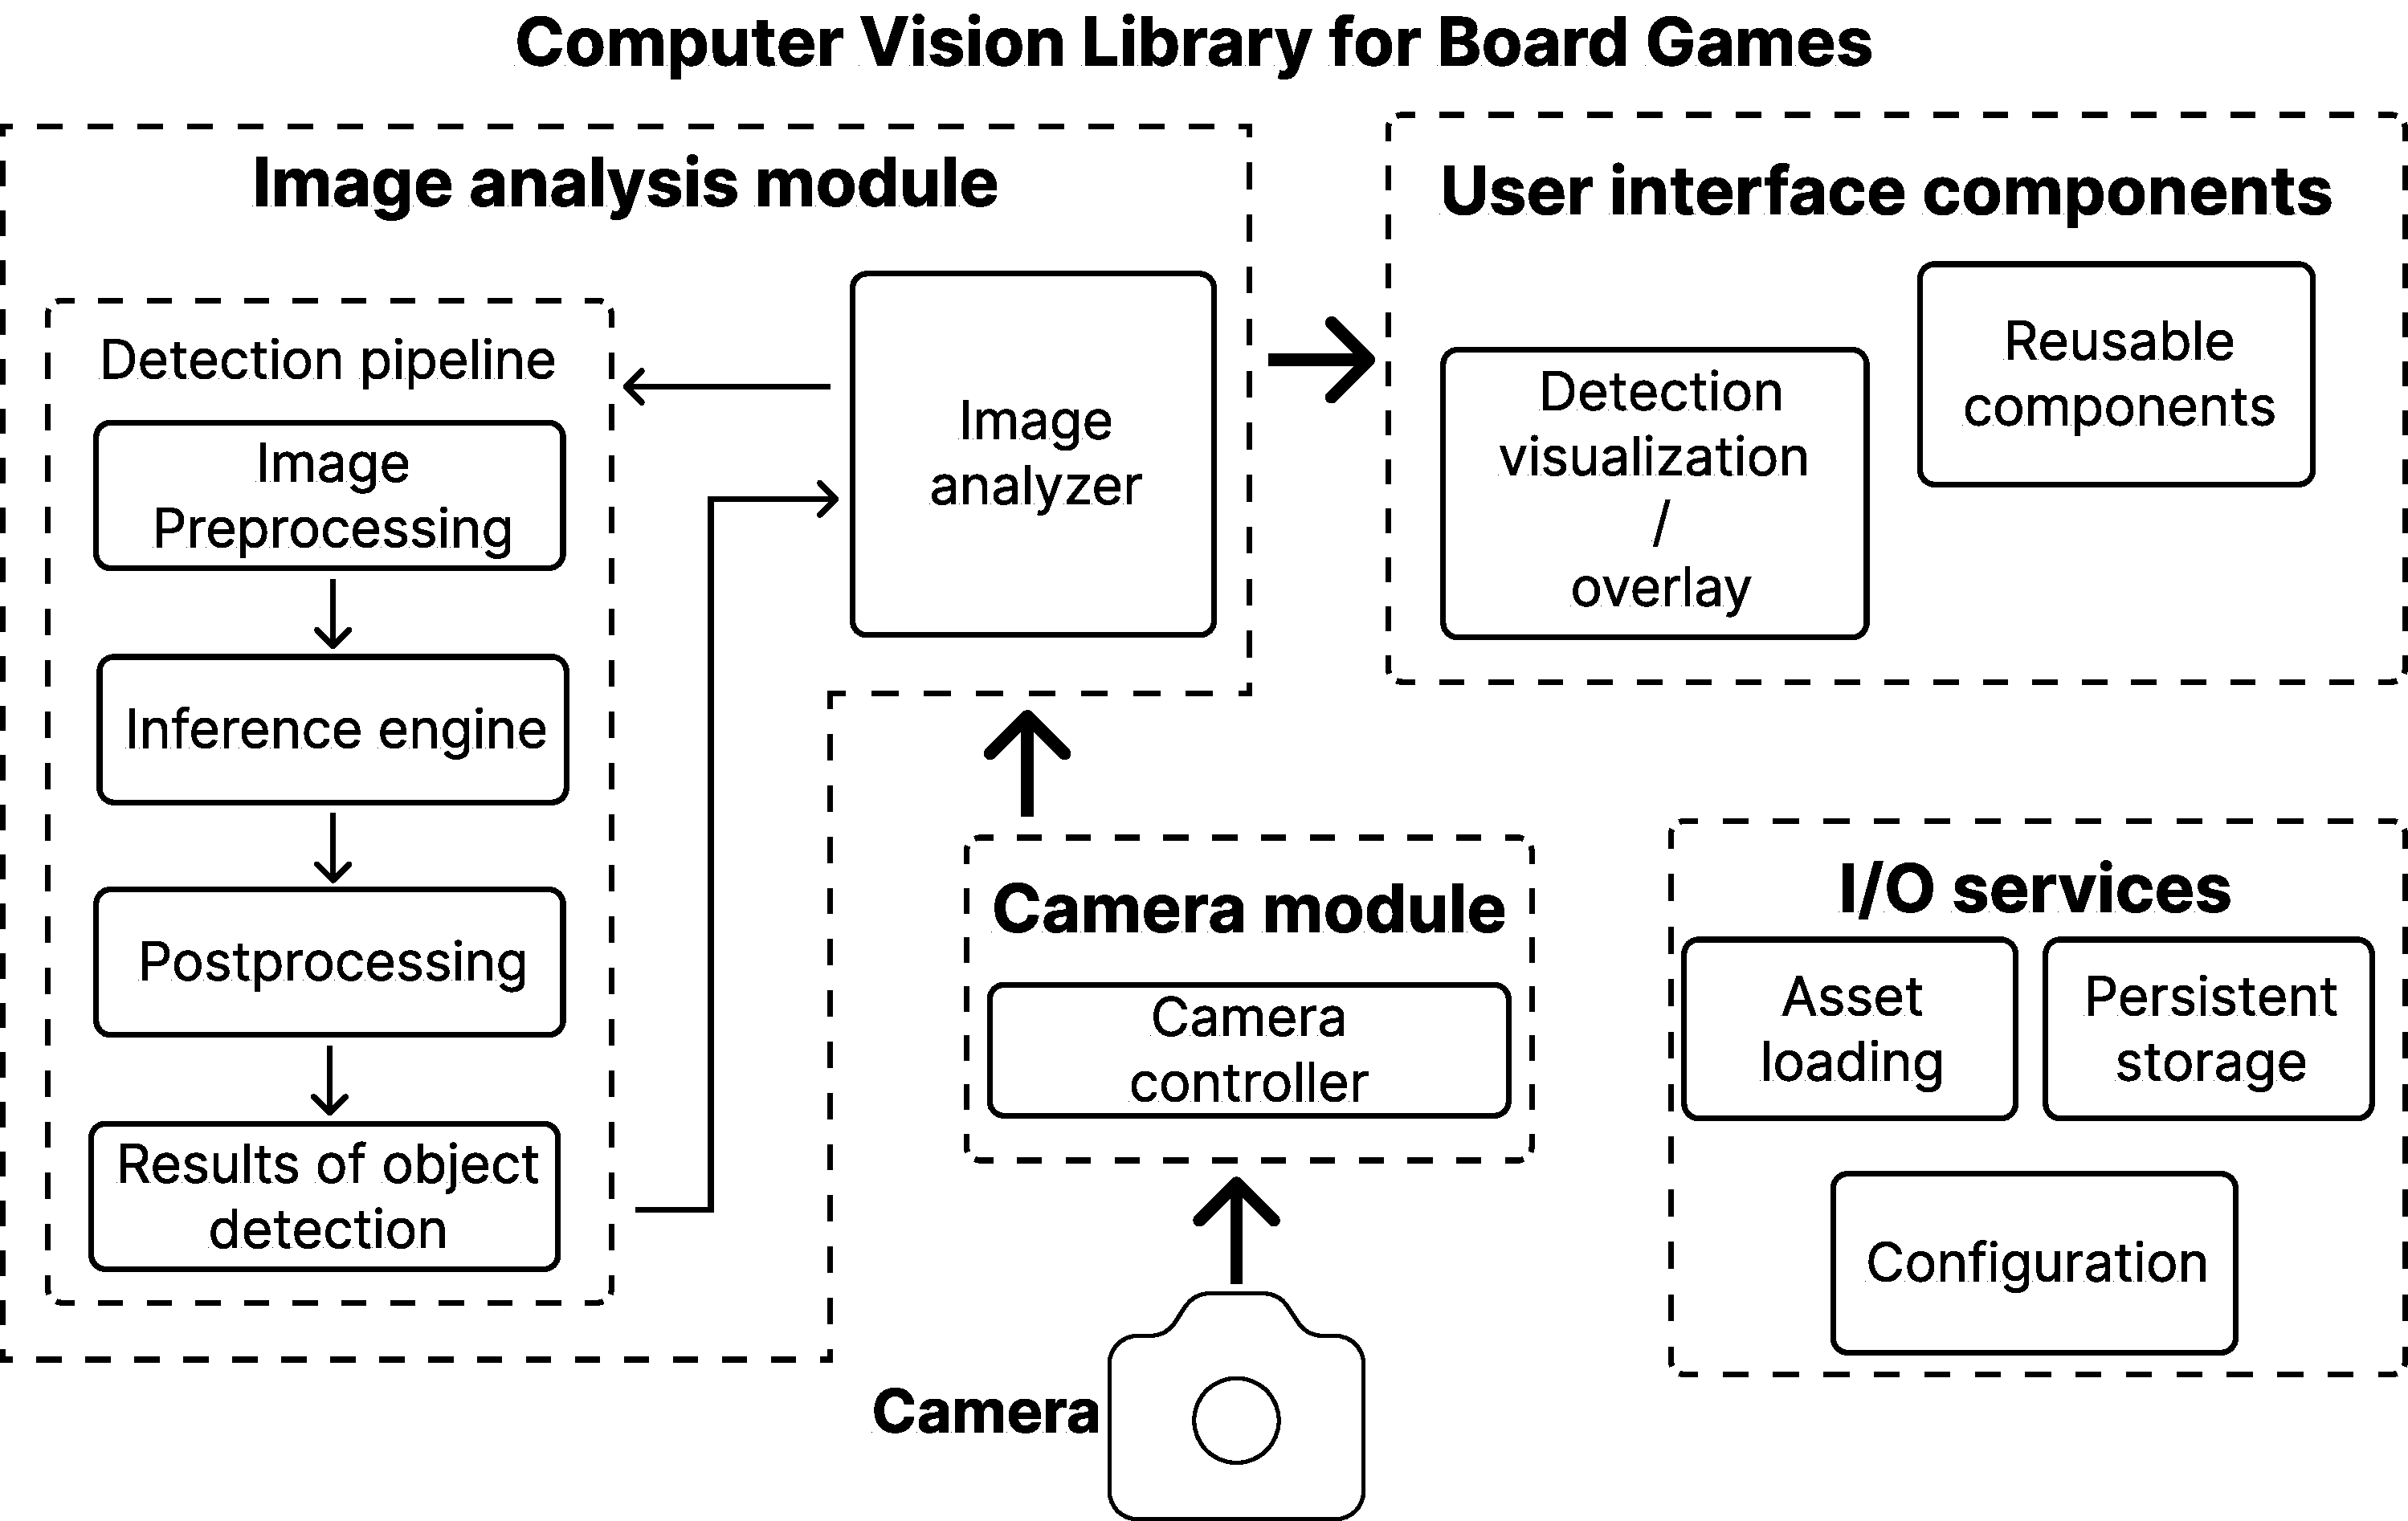
\includegraphics[width=0.8\textwidth]{obrazky-figures/cvlibg_scheme.pdf}
	\caption{Abstract scheme of mobile library separated into modules.}
	\label{cvlibgScheme}
\end{figure}

The overall structure of CVLiBG is shown in Figure ~\ref{cvlibgScheme}. The library is divided into modules that communicate with each other. The following sections will describe the modules in detail.


% =======================================================================================
The general knowledge about Android and Kotlin was mostly gained from the Kotlin documentation \cite{kotlinDocs}, the Android API documentation \cite{androidDocs}, and ARM's online course \cite{armTutorial} alongside the YouTube version of the same course \cite{armYtTutorial} for Android application development using the OpenCV camera, which was used as a starting point.
% =======================================================================================


\section{Used technologies}
This section presents the main used technologies in the implementation of the CVLiBG library, alongside the reasoning behind their selection. The chosen technologies directly influenced the design of the system, particularly camera integration, image processing, and model inference.

\subsection{Operating system}
Operating systems for mobile phones are mostly dominated by two systems: Android and iOS. Since 2020, the smartphone market share has been steadily at 70\% \cite{phoneOsStatistics} in favor of Android over iOS. For this reason, Android was chosen as the target operating system.

% ===================================
\subsection{Kotlin}
For a long time, Java was the main programming language for Android development. However, in 2019\footnote{Android's Kotlin first approach: \url{https://developer.android.com/kotlin/first}}, Google announced the introduction of the Kotlin language. The blog also highlights Kotlin's advantages, such as its easier to understand code, safer null exception handling, and exceptional concurrency handling. One of the biggest advantages of the Kotlin language is its interoperability with Java. This feature is crucial, as it allows Kotlin code to use Java code and vise versa, which means that using Kotlin results in less code overhead while keeping all the benefits and support of the Java packages created over the long duration of Java's existence. For this reason, Kotlin was chosen as the main programming language.

% ===================================
\subsection{IntelliJ Idea}
The most popular integrated development environments (hereafter referred to as IDEs) for developing applications in Android are Android Studio and IntelliJ Idea. Both IDEs are similar at first glance, as they also share internal code\footnote{JetBrains blog post on IntelliJ Idea and Android studio: \url{https://blog.jetbrains.com/idea/2013/05/intellij-idea-and-android-studio-faq/}}. While the recommended approach for Android development is to use Android Studio, I, as the author, leaned toward IntelliJ Idea due to  personal preference and previous experience.

% ===================================
\subsection{OpenCV}
OpenCV\footnote{OpenCV's about page: \url{https://opencv.org/about/}} is a multi-platform and multi-language open source library for computer vision, machine learning, image manipulation, and many more use-cases. It is a well established library used by many companies and institutions, such as NASA, ARM, JetBrains, and others. 

OpenCV was included for its wide range of computer vision algorithms utilized by CVLiBG and Dataset Creator (see \ref{datasetCreator}), which allowed re-usability, even with different programming languages. An alternative to using OpenCV would be to implement custom image manipulation algorithms or finding a suitable replacement that could be shared across two parts of this thesis. 

Furthermore, OpenCV implements an inference engine for CNN based neural networks. While this use case remained in the final version of CVLiBG, it was replaced with another module due to its superior performance.


% ===================================
\subsection{CameraX}
\label{cameraX}
The CameraX library was selected as the primary approach for camera access in this project. CameraX is a Jetpack library built on top of the Camera2 API~\cite{cameraXApi}. 

Compared to the Camera2 API, which allows low-level camera control, CameraX exposes a high level abstraction layer that simplifies camera integration in Android applications and this library. CameraX also provides predefined use cases, such as
preview\footnote{CameraX Preview: \url{https://developer.android.com/media/camera/camerax/preview}}, 
image capture, video capture, 
and image analysis\footnote{Image analysis: \url{https://developer.android.com/media/camera/camerax/analyze}}.
This abstraction eliminates the need to manually handle device-specific behavior \cite{cameraXApi}. Furthermore, CameraX uses Android lifecycle components, which simplifies resource management and reduces the risk of memory leaks.

An alternative approach was to use OpenCV's camera access. However, this approach lacks lifecycle integration, requires manual resource management, and will result in the need to design a custom data flow between the proposed \textbf{Camera module} and the \textbf{Image analysis} modules. In contrast, using CameraX simplifies this approach by using an interface.

Another important consideration is that CameraX and OpenCV use different image formats.
CameraX provides image data in the YUV\_420\_888 format, whereas OpenCV operates primarily on BGR or RGBA representations. Therefore, a conversion step is required before further processing can be performed.

The resulting design uses CameraX as the camera interface, while OpenCV is used exclusively for image processing. Despite the required conversions, this approach leverages the simplicity of CameraX together with the flexibility of OpenCV for implementing the detection pipeline.

% ===================================
\subsection{Open Neural Network Exchange}
\label{chosingInferenceRT}
The most popular and widely used inference runtimes are \textbf{TensorFlow Lite} and the \textbf{Open Neural Network Exchange Runtime} (hereinafter referred to as ONNX). Both of these runtimes are supported on mobile devices. A study from 2023~\cite{Ren2023_ONNX_TensorFlow_BScan} shows ONNX out-performing TensorFlow on both CPU and GPU. The other blog post \cite{aimtechnoOnnxTFcomparison} from 2025 shows that the difference between the two runtimes is decreasing, with ONNX being slightly faster. The study also points out the open nature of ONNX and its more multi-platform development approach, whereas TensorFlow Lite can benefit from Google's ecosystem. Because of the open nature and small performance benefits, especially on CPUs, ONNX was chosen for this library. However, it should be noted that CVLiBG was designed to be expandable, and developers can implement their preferred runtime should they decide to do so.

% =======================================================================================

% =======================================================================================

\section{Integrating CVLiBG into Android applications}
CVLiBG is designed as a library that integrates into Android applications. It does not provide its own navigation, nor does it require a specific application structure, but instead operates within existing activities or fragments.

The library interacts with the UI elements through components such as \texttt{PreviewView} 
and custom overlay views (see Section~\ref{DetectionOverlay}), which must be provided by the application. Furthermore, CVLiBG exposes Kotlin's \texttt{Flow} and callback functions, which allow further interaction with modules.

Camera access in Android requires explicit user permission, which must also be declared in \texttt{AndroidManifest.xml}\footnote{Android manifest permissions: \url{https://developer.android.com/guide/topics/manifest/manifest-intro\#perms}}. The activity that initializes the camera must request this permission. This can be achieved manually or by using the helper method from the \texttt{CommonUtils} called \texttt{checkCameraPermission()}, provided by the library.


% ======================================================================================

% ======================================================================================


\section{Camera module}
\label{CameraModule}
The camera module's responsibility is to acquire image data and provide it to the image analysis module. Its purpose is to abstract and hide camera initialization, lifecycle handling, and image data flow from the developers. In the implementation, this functionality is mainly provided by the \texttt{CameraController} class.

% ===================================
\subsection{Camera module's initialization and rebinding}
The camera module is designed to have a lightweight initialization and to be a long-lasting object. The constructor only receives the Android \texttt{Context} and an optional \texttt{ImageAnalyzer}. Expensive operations, such as obtaining the \texttt{ProcessCameraProvider}, creating CameraX use cases, initializing the camera executor, and building detectors, are delayed until the \texttt{start()} method is called.

Instead of initializing a new instance with each view creation, it is recommended to place the controller into longer lasting parts of the application, such as \texttt{ViewModel}. The \texttt{start()} method requires \texttt{LifecycleOwner} and \texttt{SurfaceProvider}, which are used to bind the current view to the \texttt{CameraController}. The first call of this method will initialize all reusable parts, while consecutive calls will rebind the use cases to a new lifecycle owner and surface provider.

This separation is especially useful for \texttt{Fragments}\footnote{Fragment lifecycle: \url{https://developer.android.com/guide/fragments/lifecycle}}, as their views can be destroyed and recreated, for example, during screen rotation, while the related \texttt{ViewModel} can remain alive. This allows the \texttt{start()} method to be called inside \texttt{onViewCreated()} and to bind existing resources to a newly created view.

The controller also provides a \texttt{stop()} method unbinding all use cases, essentially disabling the camera and analysis. This should be useful for developers who want to pause the camera, instead of relying on CameraX's automatic solution described in the next section.

% ===================================
\subsection{Camera lifecycle and resource release}
Continuous camera usage and image analysis consume processing resources and battery power. Therefore, especially on mobile devices, it must be managed carefully. Otherwise, applications that are not in use could be wasting battery in the background. To eliminate this problem, CameraX uses \texttt{ProcessCameraProvider}\footnote{Camera Provider: \url{https://developer.android.com/reference/androidx/camera/lifecycle/ProcessCameraProvider}}, which can be bound to the lifecycle and managed automatically.

In Android, the lifecycle describes the current state of an activity or fragment, such as active, paused, stopped, or destroyed. Binding the camera provider to this lifecycle allows CameraX to automatically release camera resources when the related activity or fragment is no longer active.

If the controller is stored outside of the fragment view lifecycle, for example in a \texttt{ViewModel}, it must still be explicitly destroyed when it is no longer needed. The \texttt{destroy()} method releases allocated resources, stops camera use cases, shuts down the executor, and prevents memory leaks.

% ===================================
\subsection{Preview and analysis use cases}
The camera module utilizes two camera use cases: preview and image analysis. The preview use case is bound to the lifecycle owner provided to the controller. On the other hand, the image analysis is set up as a separate use-case and moved to another thread using \texttt{ExecutorService}. This separation enables the camera preview to be a continuous stream of image data while the image analysis works separately.

% ===================================
\subsection{Frame handling}
It is expected that the camera will produce images faster than the images are being analyzed. The image analysis supports two operating modes: blocking and non-blocking. The blocking mode keeps an internal buffer of produced image data. However, this behavior would lead to old frames being analyzed while the camera has already moved. To use only the newest images, a strategy is set up inside the camera module using \texttt{ImageAnalysis.STRATEGY\_KEEP\_ONLY\_LATEST} to operate in non-blocking mode.

% ===================================
\subsection{Resolution and aspect ratio selection}
The image analysis and camera preview require the resolution at which they will operate. The resolution is determined by the detectors (see~\ref{Detector}). A higher pixel count (\texttt{width x height}) is used as the base for finding the resolution. If the camera cannot provide the requested resolution, it will fall back to the closest resolution that is higher than the required one. This achieves the lowest possible resolution, which speeds up the preprocessing of the images while losing as little detail as possible.

Object detection models, such as YOLO, which are used in this project, usually expect a \texttt{640x640} input resolution with a \texttt{1:1} aspect ratio. However, not all devices support this, or they would have to rescale the image, causing performance decreases. Furthermore, the preview will be displayed onto mobile screens, which usually do not use the \texttt{1:1} aspect ratio. Based on the statistics~\cite{aspectRatioStats}, the most common, or rather the closest to it, is \texttt{16:9}. Other supported options, such as \texttt{4:3}, would likely waste performance as the excess will be cropped from the screen.

% =========================================================================================

% =========================================================================================
\section{Image analysis module}
The responsibility of the image analysis module is to receive image data from the camera module, coordinate its analysis, and expose the resulting data to the rest of the application. The actual image analysis is performed by the \texttt{Detector} classes described in the following section. The implementation of the image analysis module is provided by the \texttt{ImageAnalyzer} class. 

This module is not, by design, lifecycle aware, meaning it has to manually acquire and release resources. However, the camera module, by default, does this automatically. This behavior can be changed with the \texttt{manageAnalyzer} parameter of \texttt{CameraController} set to false.


\subsection{Frame analysis}
The \texttt{ImageAnalysis} use case, mentioned in the camera module, can be set up with an \texttt{ImageAnalysis.ImageAnalyzer}, an interface that is implemented by this module/class. This connection automatically handles data flow from the camera to the \texttt{ImageAnalyzer} class. As an implementation of the \texttt{ImageAnalysis.ImageAnalyzer} interface, this class defines the \texttt{analyze()} method with a single input parameter, \texttt{ImageProxy}. These objects contain the image data, as well as the camera rotation, data format, etc. 

It should be noted that during the initialization of image analysis in the camera module, the use case was set up to automatically convert input image data from YUV format to RGBA format, as well as to automatically rotate the image data. These options slow down image analysis; however, they also simplify the design.

The analyzer also prevents overlapping analysis runs. If a previous frame is still being processed, or if analysis is paused, the incoming \texttt{ImageProxy} is closed immediately and the frame is skipped.

% ===================================
\subsection{Analysis modes}
Image analysis module uses two detectors derived from the abstract \texttt{Detector} class. These detectors take an image bitmap as input and output the results of these operations. The \texttt{ImageProxy} is converted into a bitmap, which is handled by the \texttt{ImageAnalyzer} to shield detectors from the responsibility of closing it. Unclosed image proxy objects will create memory leaks. Furthermore, \texttt{ImageAnalyzer} contains logic for switching between two operating modes, each using a different detector. 

\textbf{Realtime} mode analyzes input data as fast as possible. This mode does not synchronize with the camera preview, which means that the projected outputs are always from the "past". Therefore, it is recommended to use lightweight models with small latency for the \texttt{realtimeDetector} used in this mode.

On the other hand, the \textbf{detailed} mode will, upon activation, analyze the first image, pause image analysis, and output the image analysis alongside the input image. Results containing detected objects, as well as the input image, can be collected and displayed by the UI or other use cases. Therefore, instead of analyzing camera inputs as fast as possible, it analyzes a single image, like a photo. This mode uses \texttt{detailedDetector} provided to \texttt{ImageAnalyzer} in its constructor.

Switching between the two modes can be achieved with \texttt{switchToDetailedAnalysis()} and \texttt{switchToFasterAnalysis()} methods.

% ===================================
\subsection{Result distribution and metrics}
\texttt{ImageAnalyzer} exposes its outputs using Kotlin's \texttt{StateFlow}\footnote{Kotlin flows on Android: \url{https://developer.android.com/kotlin/flow}} \footnote{StateFlow Android Guide: \url{https://developer.android.com/kotlin/flow/stateflow-and-sharedflow}}. Unlike simpler approaches, such as callback functions, this approach allows multiple data consumers across different threads while maintaining thread safety. Exposed \texttt{detectionResult} contains the results of image analysis, and \texttt{metrics} contains performance and additional metrics. 

The main exposed value is \texttt{detectionResult}, which contains the latest \texttt{DetectorResult} produced by the active detector. This result can be consumed by user interface components, such as \texttt{DetectionOverlay}, or by application-specific logic. In detailed analysis mode, the emitted result may also contain the analyzed input image, allowing the user interface to display a frozen frame together with the detected objects.

The second exposed value is \texttt{metrics}, which contains an \texttt{AnalyzerMetrics} object. This object combines the total analysis time, timing values, and additional detector metrics. These values can be displayed using \texttt{MetricsOverlay} or used during development to compare detectors and identify performance bottlenecks.

Metrics can be enabled with the \texttt{setMetricsEnabled()} method, and for verbose metrics, using the \texttt{setVerboseMetricsEnabled()} method.

When using this data inside UI fragments or activities, it is required to use lifecycle aware code that resets when the view is being destroyed; otherwise, this behavior may lead to application crashes.


% ===================================
\subsection{Concurrency and coroutines}
\label{concurrencyExplained}
Real-time image analysis requires concurrent processing since camera frames are continuously delivered while detection and UI updates must not block the main thread. To achieve this, CVLiBG utilizes Kotlin's concurrency handling, achieved with relatively low code overhead. Kotlin allows developers to write asynchronous code in a sequential style. This language feature abstracts away much of the complexity associated with thread management \cite{kotlinConcurrency}.

Non-blocking context switching is achieved with the \texttt{withContext} function, which allows the code inside a coroutine to switch to different contexts while maintaining the sequential code style. Coroutines use dispatchers, which schedule execution threads or a pool of threads. The most commonly used dispatchers are \texttt{Main}, \texttt{IO}, and \texttt{Default}. The \texttt{Main} dispatcher is used for executing code on the main thread, which also manages the UI. Usually, manipulating UI elements outside of the main thread results in a runtime exception. The \texttt{Default} thread pool is used for CPU-heavy computations, such as the benchmarks described later that can take a few minutes to complete. The last dispatcher is for input and output operations.

Kotlin also allows developers to group coroutines using a principle called structured concurrency. This principle treats coroutines as a hierarchical tree of parent and child tasks. These so-called scopes allow coroutines to define lifecycle boundaries and manage coroutines within the scope \cite{kotlinConcurrency}.


% ===============================================================================

% ===============================================================================


\section{Object detection pipeline}
\label{Detector}
The object detection pipeline is mostly represented by the \texttt{Detector} class. Its purpose is to process the input image, perform object detection analysis, and return structured outputs. The implementation of internal analysis is up to the developer; however, its inputs and outputs should always be the same. This approach allows image analysis to remain reusable, even for different implementations.

% =========================================
\subsection{Abstract Detector}
All detectors must be derived from the abstract \texttt{Detector} class. This class enforces the inputs and outputs of the detectors, as well as the initialization and building of the detectors; the rest is up to the developers.

The \textbf{inputs} of the detector are always bitmaps in RGBA format and have a resolution provided by the camera. Should developers need to change this, such as a different data format, it would require rewriting \texttt{ImageAnalyzer}.

\textbf{Initialization}, or rather the constructor of detectors, should always contain the path to the model inside the project's assets directory and the required input resolution of the model. This design ensures that the initialized detectors have low memory usage until they are built and used. 

The detector becomes usable once it is \textbf{built} using the \texttt{build()} method. This method requires context for loading models from the project's asset folder. Developers must implement the \texttt{runtimeSetup()} method, which prepares models for executing object detection task. Should the models be used without building them first, a guard will throw an \texttt{IllegalStateException}. 

% =========================================
\subsection{Implemented detectors}
As mentioned before, this library uses OpenCV's image manipulation algorithms. OpenCV also contains the \texttt{Dnn} package, which can be used as an inference runtime. This approach, however, was replaced by ONNX's Runtime, which, based on testing, provides almost 2 times faster inference. 

The key idea of CVLiBG is to be modular and reusable. However, it should not force developers into loading unwanted modules should they decide not to use them. Because of that, ONNX's implementation of detectors was separated into another module. This enables developers to use CVLiBG and implement their own detectors or use OpenCV's predefined implementation without the need for an additional ONNX library that may not be utilized. The list of predefined detectors from both modules:

\begin{itemize}
  \item {\texttt{AbstractYoloDetector} is an abstract class containing common methods and algorithms for all YOLO-based detectors.}
  \item{\texttt{YoloOpenCV} uses OpenCVs \texttt{Dnn} inference engine. It supports YOLO version from 8 to 11 and extends the \texttt{AbstractYoloDetector}.}
  \item {\texttt{YoloOnnxDetector} is based on \texttt{AbstractYoloDetector} and is usable for YOLO models from version 8 to version 11. The detector uses the ONNX runtime as an inference engine.}
  \item {Yolo26OnnxDetector is a specialized version of \texttt{YoloOnnxDetector} for YOLO26 version.}
\end{itemize}
\bigskip


% =====================================
\subsection{Preprocessing implementation}
As mentioned before in section~\ref{imagePreprocessing}, image data needs to be processed before it can be used in inference engines. Both implemented solutions, OpenCV's and ONNX's, utilize almost identical preprocessing steps and algorithms, shared from the \texttt{AbstractYoloDetector} class.

The first step of preprocessing is converting input data from Kotlin's \texttt{Bitmap} to the OpenCV's \texttt{Mat} object. This allows the use of OpenCV's image manipulation methods and algorithms going forward. 

Models used in this project require an input resolution of \texttt{640x640} pixels. Therefore, it is necessary to resize them to the desired resolution. The method used is identical to the one described in \ref{letterboxing}, while utilizing OpenCV's \texttt{Imgproc.resize()} for resizing and \texttt{Core.copyMakeBorder()} method for letterboxing. The used padding value \texttt{(114, 114, 114)} follows the default letterboxing convention used by Ultralytics YOLO implementations, where 114 is used as a neutral gray padding value.

The last step changes based on the implemented detector. OpenCV's detector uses the \texttt{Dnn.blobFromImage()} method to convert an RGB \texttt{Mat} into a 4-dimensional blob (also Mat) used by OpenCV's inference engine. This step normalizes RGB values into float values.

The ONNX based detector, likewise, normalizes the letterboxed image. The next step converts the image from HWC format into CHW format (explained in~\ref{hwcAndChwFormats}). This is achieved by splitting the image into channels, using OpenCV's \texttt{Core.split()} method and copying this data into a new array in CHW format. Lastly, an ONNX's \texttt{OnnxTensor} object is created from the newly reordered data.

% =====================================
\subsection{Postprocessing implementation}
After preprocessing, the data is passed in their respective forms, into ONNX's \texttt{OrtSession} and OpenCV's \texttt{Dnn.Net}, respectively. The output of both inference runtimes is similar, using different objects to represent it. OpenCV uses \texttt{Mat}, whereas the ONNX library uses \texttt{OrtSession.Result}. Both outputs are flattened, as they are usually 3-dimensional (see~\ref{postprocessing}) and converted to 1-dimensional float arrays. 

The next step creates a list of \texttt{Detection} objects using the \texttt{extractDetectionResults()} method, implemented in \texttt{AbstractYoloDetector}. This method extracts attributes of each detection using the \texttt{[attributes]x[detections]} memory format explained in \ref{readingDataFormats}. A thresholding filter is applied during this step, where detections with low confidence are removed. Detection objects are also scaled back to the input dimensions of the image.

The last part of the postprocessing is Non-Maximum Suppression. OpenCV uses its \texttt{Dnn.NMSBoxes()} method to perform NMS. However, this method requires an array of OpenCV's \texttt{Rect2D} objects. Therefore, a conversion from CVLiBG's \texttt{Detection} object is required.

On the other hand, ONNX uses the custom NMS \texttt{cvlibgNmsFilterByClass()} method that works directly with \texttt{Detection} objects. Objects are grouped by their class to prevent inter-class elimination of objects. Next, detections are sorted by their confidence scores. Lastly, an implementation of NMS in Kotlin's language is applied. Both NMS and Intersection over Union algorithms are based on the \cite{opencvNMS}.

% =====================================
\subsection{Representation of detection results}
The result of the detection pipeline is always a \texttt{DetectorResult} object. This data class contains a list of detected objects (\texttt{Detection} objects), image details, the input image, and metrics.

The image details are represented by the \texttt{ImageDetails} data class. It holds information about the scaling applied during resizing and the padding values applied for each dimension. Both implemented detectors scale the detected objects back to the dimensions of the input image; however, not all implementations might require this. Therefore, the image details class provides a way for developers to scale back detections, even outside of the \texttt{Detector}.

The input image is not included by the detector itself; it is added by the \texttt{ImageAnalyzer} for use by \texttt{DetectionOverlay}.

Lastly, the metrics are an optional part of the \texttt{DetectorResult}. Detectors can provide performance metrics represented as a map of \texttt{TimerResult} objects, a small helper class containing measured time in nanoseconds, or a list of \texttt{MetricsValue} objects containing various metrics.

\subsection{Detector registry}
\label{DetectorRegistry}
It is reasonable to assume that most consumer applications will use a predefined set of object detection models and will not allow users to change them. However, some applications may require switching between models or detector implementations, either manually or automatically, based on collected metrics.

Detector implementations are often compatible with multiple models, as long as the model input and output formats remain the same. For example, the ONNX-based detectors support different YOLO model sizes and can switch between execution providers, from CPU to Google's Neural Networks API\footnote{Neural Networks API: \url{https://developer.android.com/ndk/guides/neuralnetworks}}, based on constructor parameters. This flexibility allows a single detector implementation to be reused with multiple models.

However, this also introduces a risk where detectors might be used with incompatible models. The \texttt{DetectorRegistry} is designed to reduce this risk by providing developers with a singleton registration process. The registry stores a key, model path, and detector factory function, allowing compatible detector instances to be created when needed.

\begin{lstlisting}
    DetectorRegistry.register("Register key", "model_path.model_extension")
            { path -> YoloOnnxDetector(path, applyNMS = false) }
\end{lstlisting}
Creating the \texttt{Detectors} can be achieved with:
\begin{lstlisting}
    DetectorRegistry.createDetector("Register key")
\end{lstlisting}

Since the registry stores factory functions instead of already built detectors, model loading and runtime initialization are still delayed until the detector is built. This keeps memory usage low and preserves the lightweight aspect of this solution. Optional detector parameters, such as confidence thresholds or NMS settings, can be configured directly inside the factory function.

% ========================================================================================

% ========================================================================================

\section{User interface overlays}
\label{DetectionOverlay}
\label{UserInterfaceComponents}

The user interface overlays of CVLiBG are responsible for presenting detection results to the user. The components provided by the library are \texttt{DetectionOverlay} and the more developer-focused \texttt{MetricsOverlay}. 

The class provides a default visualization; however, it is designed to be extended so that applications can adapt the appearance, displayed information, and interaction style to their specific use case.

\subsection{Detection visualization}
\label{DetectionOverlay}

The \texttt{DetectionOverlay} class provides a visualization of detected objects and an interface for interacting with these detections. The class itself provides a default implementation; however, it is designed to be extended so that applications can adapt the appearance, displayed information, and interaction style to their specific use case.

It is implemented as a transparent layer rendering detected objects on top of the camera preview (see~\ref{CameraFragmentOverlays}). Its default implementation draws detected objects using the \texttt{drawDetections()} method.

The overlay also supports drawing the analyzed image as a background. This feature is mainly used in detailed analysis mode, where the image analysis module captures a single frame, waits for a slower detector to finish processing it, and then displays both the frozen image and the resulting detections.

\subsection{Coordinate transformations}
\label{coordinateTransoformations}
Camera resolution, output dimensions of models, and screen resolutions. These three resolutions are usually not the same, and a mismatch will result in detections not aligning with the objects on the camera preview. 

To fix a resolution mismatch caused by the preprocessing of the image before inference, an \texttt{ImageDetails} object should be used if the \texttt{Detector} doesn't do it automatically.

Image details also include input image resolution, as these cannot be inferred solely from the scale. These values are used to fix the camera and screen resolution mismatch. Using the \texttt{scaleDetectionToScreenRect()} method, detections are scaled to the screen dimensions instead of the camera dimensions. 

This method, however, assumes that the \texttt{PreviewView} used to display the camera preview uses the \texttt{ScaleType.FILL\_CENTER} scale type. This option scales the preview to the screen while keeping the aspect ratio, cropping one of the dimensions (width or height) to fit the screen. This approach is recommended; other approaches might require changing the \texttt{DetectionOverlay} implementation.

\subsection{Metrics visualization}
The library also provides the \texttt{MetricsOverlay} view, which is intended mainly for development and debugging. This component visualizes metrics from image analysis. Unlike \texttt{DetectionOverlay}, which is meant to be visible to end users, \texttt{MetricsOverlay} is primarily a diagnostic tool for developers.


\subsection{Required UI layout}
\label{CameraFragmentOverlays}
The camera fragment or activity containing the preview, detection overlay, and metrics overlay is required to place the preview and overlays on top of each other with the same size in order for detections to be visible on top of the \texttt{previewView}. This implementation assumes the \texttt{ScaleType.FILL\_CENTER} is used, as mentioned in \ref{coordinateTransoformations}. 

\begin{figure}[hbt]
	\centering
	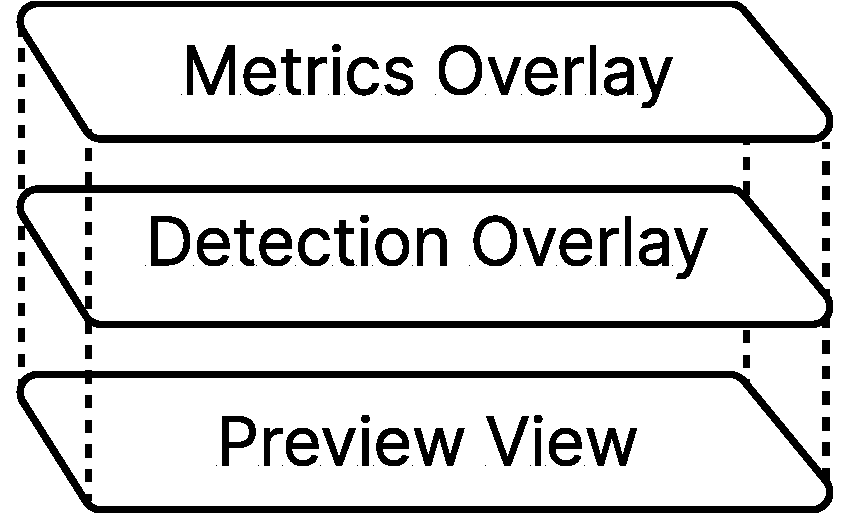
\includegraphics[width=0.4\textwidth]{obrazky-figures/camera_fragment_overlay.pdf}
	\caption[Camera preview, detection overlay, metrics layout]{Layout of user interface elements required by the \texttt{CameraController} where detections are on top of the preview of the camera.}
\end{figure}


% ===========================================================================================

% ===========================================================================================

\section{Input and output services}
\label{Services}

CVLiBG provides several input and output services used for loading assets, reading configuration files, and storing application data. These services are intended to reduce repeated boilerplate code in applications that use structured JSON files. The services are based on serializable Kotlin data classes and use the \texttt{@Serializable}\footnote{Kotlin's serialization: \url{https://kotlinlang.org/docs/serialization.html}} property.

Implemented services differ in their storage location and intended use. However, they share the same general design. Each service works with a target file or directory path, a serializer generated by the data class, and a character set used for reading or writing data.

\subsection{Configuration service}
\label{ConfigService}

The configuration service is intended for loading and storing configuration files in JSON format. These files are stored inside the application's internal folder structure, which is beneficial for storing sensitive data, such as internal configurations that should generally not be changed using external tools. The provided \texttt{filename} parameter may point to a non-existing file; this file will be created on the next \texttt{save()} method call. Furthermore, this service requires a lambda function that returns a default value if the file is not found.

\subsection{Asset service}
\label{AssetService}
\texttt{AssetService} is used for loading JSON files from the assets folder. These files are read only. The loaded JSON file must contain a list of objects instead of a single JSON object. These objects will be loaded into memory as a map for faster look-up. Because of that, it is required to define a \texttt{keySelector}, which will be used as a key for the internal map look-ups. 

The \texttt{path} parameter of this service can be a directory, which will apply a recursive search to look for all JSON files. These will be joined to an internal map. Repetitive keys will be overridden, an error will be printed to the console, and an \texttt{onRepetitiveKeyError} callback will be invoked if it is defined.

Recursive search with multiple files provides developers with the option of separating loaded objects into groups for easier data editing; however, the JSON objects must be of the same \texttt{data class} type. Lastly, the values are \textit{lazily} evaluated on the first attempt to read them.

\subsection{Storage service}
\label{StorageService}
The storage service allows loading and saving a single JSON file, containing a list of JSON objects. Unlike the \texttt{AssetService}, it uses external storage. This location is preferred for storing logs or other data, as it can be accessed using the system file manager or when the mobile device is connected to a computer. 

Service requires \texttt{keySelector} for deciding which element of the \texttt{data class} will be used as a key for the map, used for internal storage of items. Furthermore, the loaded file does not have to exist and can be created by the service upon saving. If the \texttt{throwOnFail} is set to \texttt{TRUE}, an exception will be thrown for the non existing file.
% ===========================================================================================

% ===========================================================================================

\section{Performance benchmarking}
CVLiBG includes a performance benchmark utility intended for comparing different models and detector implementations. This is implemented by the \texttt{PerformanceBenchmark} class. This benchmark uses a constant input image and performs multiple inference runs for the specified detector/model combination. This class provides a simple way for developers to benchmark models and export the results into the \texttt{.csv} format.

This is important, as different models and architectures for object detection may differ in performance depending on the device hardware. It is generally accepted that GPU and NPU acceleration are preferred for executing neural networks, especially object detection models. However, performance depends on hardware support and model compatibility, and some devices, especially budget ones, may not benefit from hardware acceleration. Based on the experiments performed in Chapter \ref{bangTrainingExperiments}, some models performed better on CPU than when using Android’s Neural Network API.